\chapter{Wdrożenie i testowanie aplikacji klienckiej}

\section{Wdrożenie aplikacji klienckiej}
\subsection{Konfigurowanie środowiska wirtualnego}
Aplikacja kliencka została stworzona jako aplikacja webowa z wykorzystaniem platformy programistycznej \textit{Angular 2}. By móc skorzystać z tego frameworku należy odpowiednio skonfigurować środowisko.

W pierwszej kolejności wymagane jest zainstalowanie środowiska uruchomieniowego Node.js, które zaprojektowane zostało do tworzenia wysoce skalowalnych aplikacji internetowych, szczególnie pod kątem serwisów www napisanych w języku JavaScript. \'Srodowisko to jest dostępne do pobrania ze strony internetowej node.js [6]. Bądź też jak to zostało wykonane w ramach projektu na systemie operacyjnym Ubuntu 16.04 poprzez komendy na listingu~\ref{lst:node}.

\lssetdef
\lstinputlisting[captionpos=b,caption={Instalacja Node.js w systemie operacyjnym Ubuntu 16.04},label={lst:node},basicstyle={\footnotesize\ttfamily}]{rozdzial06/node.txt}

Kolejnym krokiem jest instalacja Angular-CLI poprzez komendy z listingu~\ref{lst:angular}

\lssetdef
\lstinputlisting[captionpos=b,caption={Instalacja Angular-CLI w systemie operacyjnym Ubuntu 16.04},label={lst:angular},basicstyle={\footnotesize\ttfamily}]{rozdzial06/angular2.txt}

Tak przygotowane środowisko umożliwia już uruchomienie aplikacji klienckiej. By uruchomić aplikację na \textit{localhost:4200} w przeglądarce internetowej wystarczy będąc w katalogu z aplikacją wydać polecenia z listingu~\ref{lst:localhost}. W tym przypadku polecenie pierwsze odpowiedzialne jest za przebudowanie projektu i wymagane jest jedynie w przypadku dodania do projektów nowych pakietów.

\lssetdef
\lstinputlisting[captionpos=b,caption={Uruchomienie aplikacji na localhost:4200 16.04},label={lst:localhost},basicstyle={\footnotesize\ttfamily}]{rozdzial06/localhost.txt}

\subsection{Zmiana domyślnego portu działania aplikacji}
Zmiana portu umożliwia uruchomienie projektu na serwerze, tak by mógł być widoczny bądź w sieci lokalnej bądź globalnie. \\

W tym celu w głównym katalogu aplikacji umieszczony został plik \textit{server.js} oraz katalog \textit{server}, w którym z kolei umieszczony został plik \textit{api.js}\\

Na listingu~\ref{lst:server} przedstawiona została zawartość pliku server.js. Numer portu na jaki został przekierowany serwis ustawiony został w 29 linii pliku.

\lssetdef
\lstinputlisting[captionpos=b,caption={Zawartość pliku server.js},label={lst:server},basicstyle={\footnotesize\ttfamily}]{rozdzial06/server.txt}

\lssetdef
\lstinputlisting[captionpos=b,caption={Zawartość pliku api.js},label={lst:api},basicstyle={\footnotesize\ttfamily}]{rozdzial06/api.txt}

Po utworzeniu tych plików uruchomienie aplikacji klienckiej na nowym porcie odbywa się poprzez komendę z listingu~{lst:run}.

\lssetdef
\lstinputlisting[captionpos=b,caption={Uruchomienie aplikacji klienckiej na własnym porcie},label={lst:run},basicstyle={\footnotesize\ttfamily}]{rozdzial06/run.txt}

\subsection{Wdrożenie API REST-owego}
Do poprawnego działania aplikacji potrzebne jest również API REST-owe pośredniczące w komunikacji aplikacji klienckiej z rozproszoną bazą danych. Podczas wdrażania projektu na systemie operacyjnym Ubuntu 16.04, API zostało umieszczone na serwerze HTTP- \textit{APACHE2}.

\section{Testy działania aplikacji}

W tej części zostały zamieszczone obrazy działania wprowadzonej aplikacji, a tym samym również poprawność działania replikacji między węzłami rozproszonej bazy danych. Aplikacja działa poprawnie i zgodnie z przewidywaniami. \\

Tak jak to już zostało wspomniane w podrozdziale \ref{chap:testReplikacji}, by replikacja mogła przebiegać prawidłowo, bazy na węzłach \textit{slave} muszą być spójne z bazą na węźle \textit{master}, a co z tego poniekąd wynika bazy na wezłach \textit{slave} muszą być utworzone i muszą posiadać taką samą strukturę tabel.

\subsection{Dodawanie rekordu do rozproszonej bazy danych}
Na rysunkach od \ref{fig:addFilm} do \ref{fig:endAddFilm} zademonstrowane zostało działanie replikacji na przykładzie dodawania filmu do bazy z poziomu aplikacji webowej.\\

Na rysunku \ref{fig:addFilm} wpisane zostały dane przykładowego filmu, a po naciśnięciu przycisku 'Dodaj film' aplikacja poprzez API REST łączy się z węzłem master rozproszonej bazy danych, gdyż wprowadzana będzie modyfikacja, a następnie dodaje dane do tabeli Filmy (rysunek \ref{fig:FilmMaster}) dzięki procedurze SQL 'DodajFilm'. Wykonana procedura zostaje replikowana do wszystkich węzłów Slave. Tabela Filmy dla wybranego węzła Slave na porcie 8083 została pokazana na rysunku \ref{fig:FilmSlave}. Z węzła Slave również odczytywane są dane poprzez aplikację kliencką, a poprawnie odczytane dane z takiego węzła zostały przedstawione na rysunku \ref{fig:endAddFilm}.

\begin{figure} [H]
	\centering
	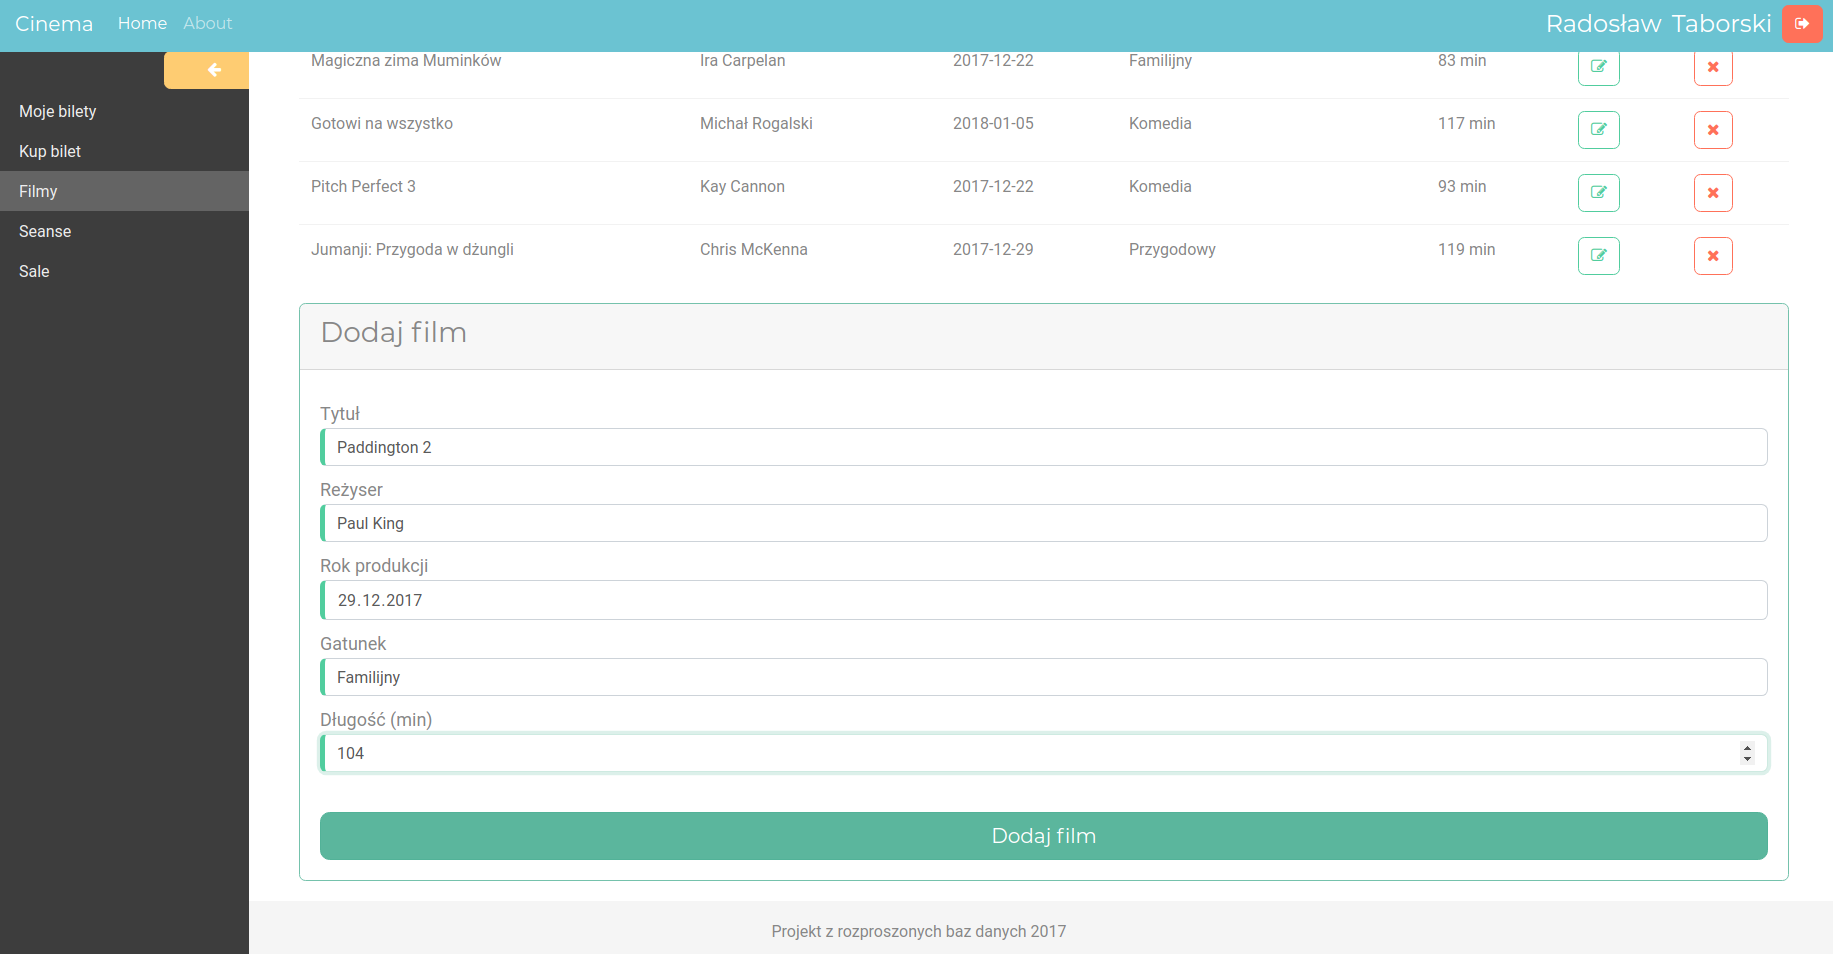
\includegraphics[width=1\linewidth]{rozdzial06/5.png}
	\caption{Dodawanie nowego filmu poprzez aplikację}
	\label{fig:addFilm}
\end{figure}

\begin{figure} [H]
	\centering
	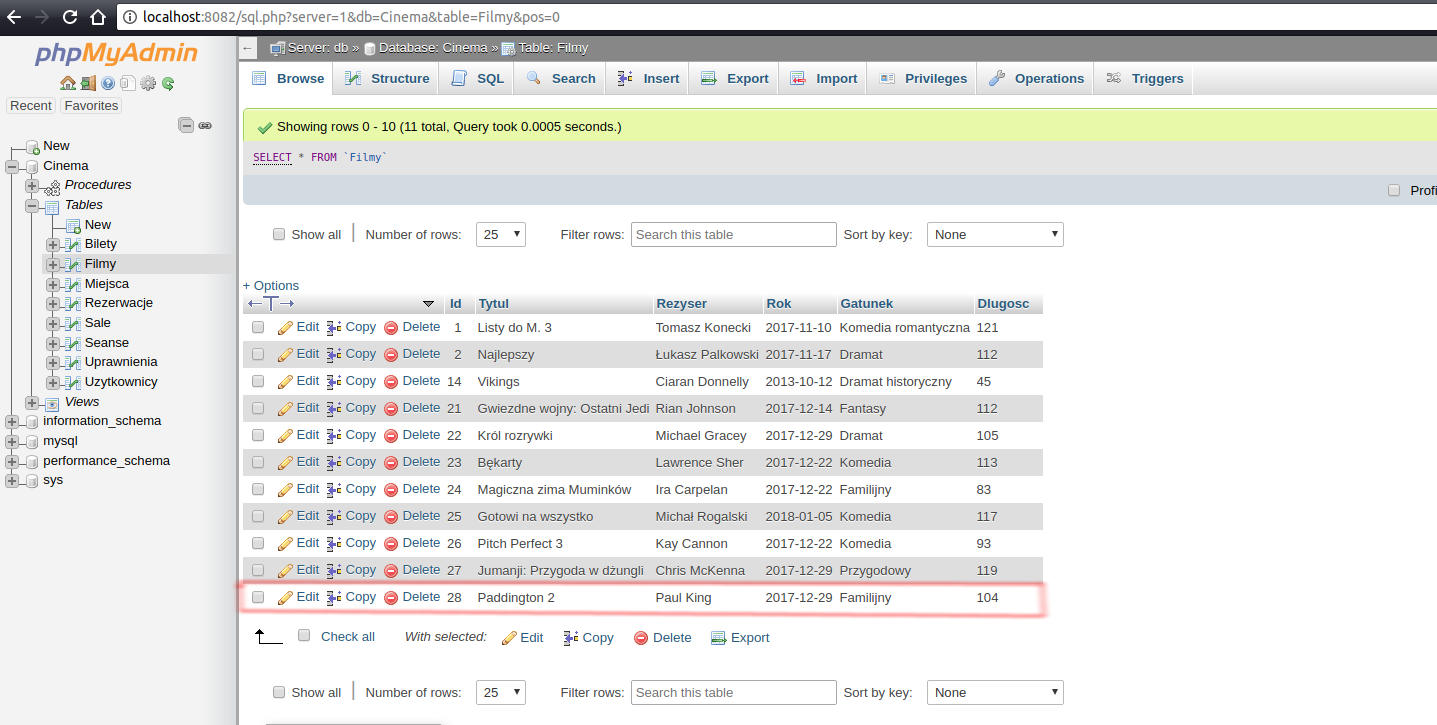
\includegraphics[width=1\linewidth]{rozdzial06/7.png}
	\caption{Tabela Filmy na węźle \textit{master} o porcie 8082}
	\label{fig:FilmMaster}
\end{figure}

\begin{figure} [H]
	\centering
	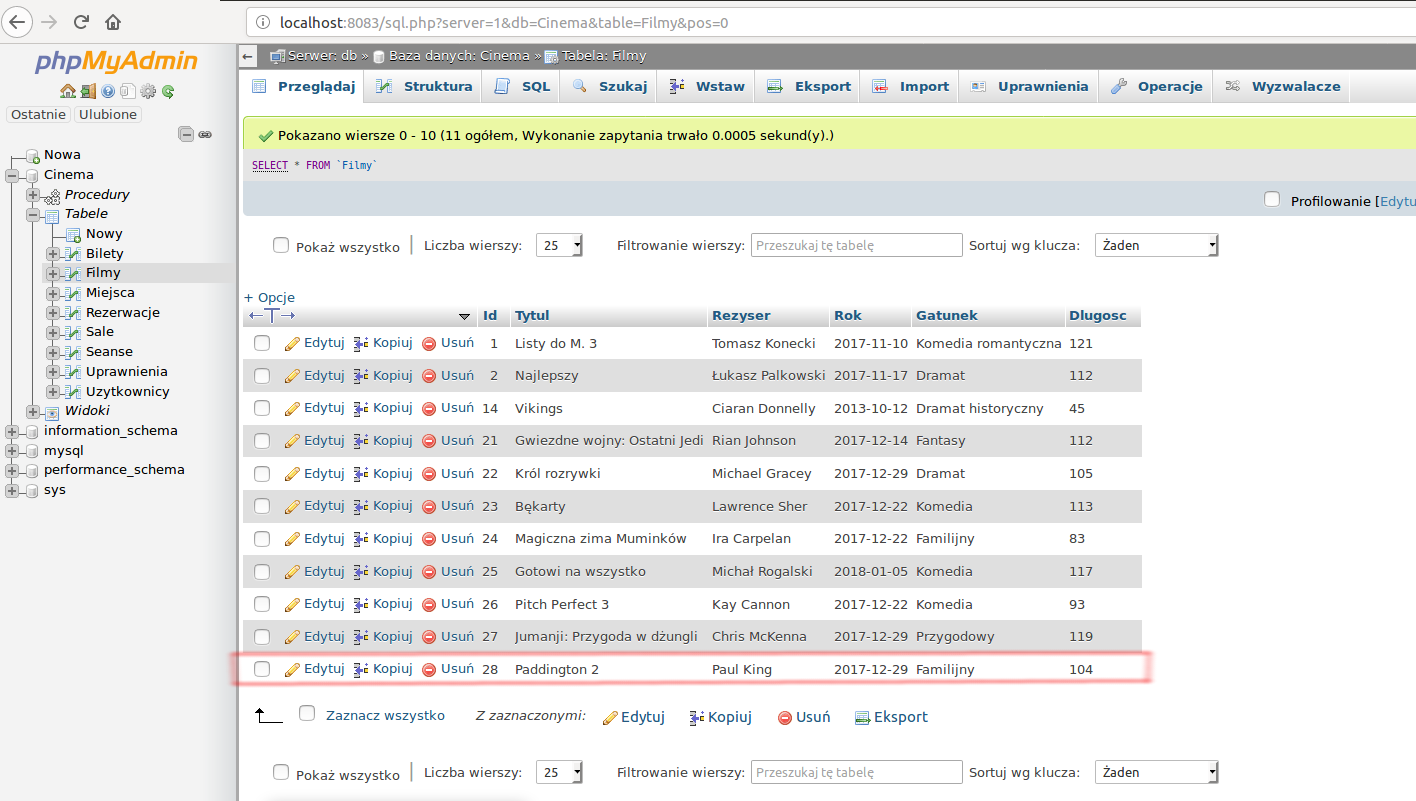
\includegraphics[width=1\linewidth]{rozdzial06/8.png}
	\caption{Tabela Filmy na węźle \textit{slave1} o porcie 8083}
	\label{fig:FilmSlave}
\end{figure}

\begin{figure} [H]
	\centering
	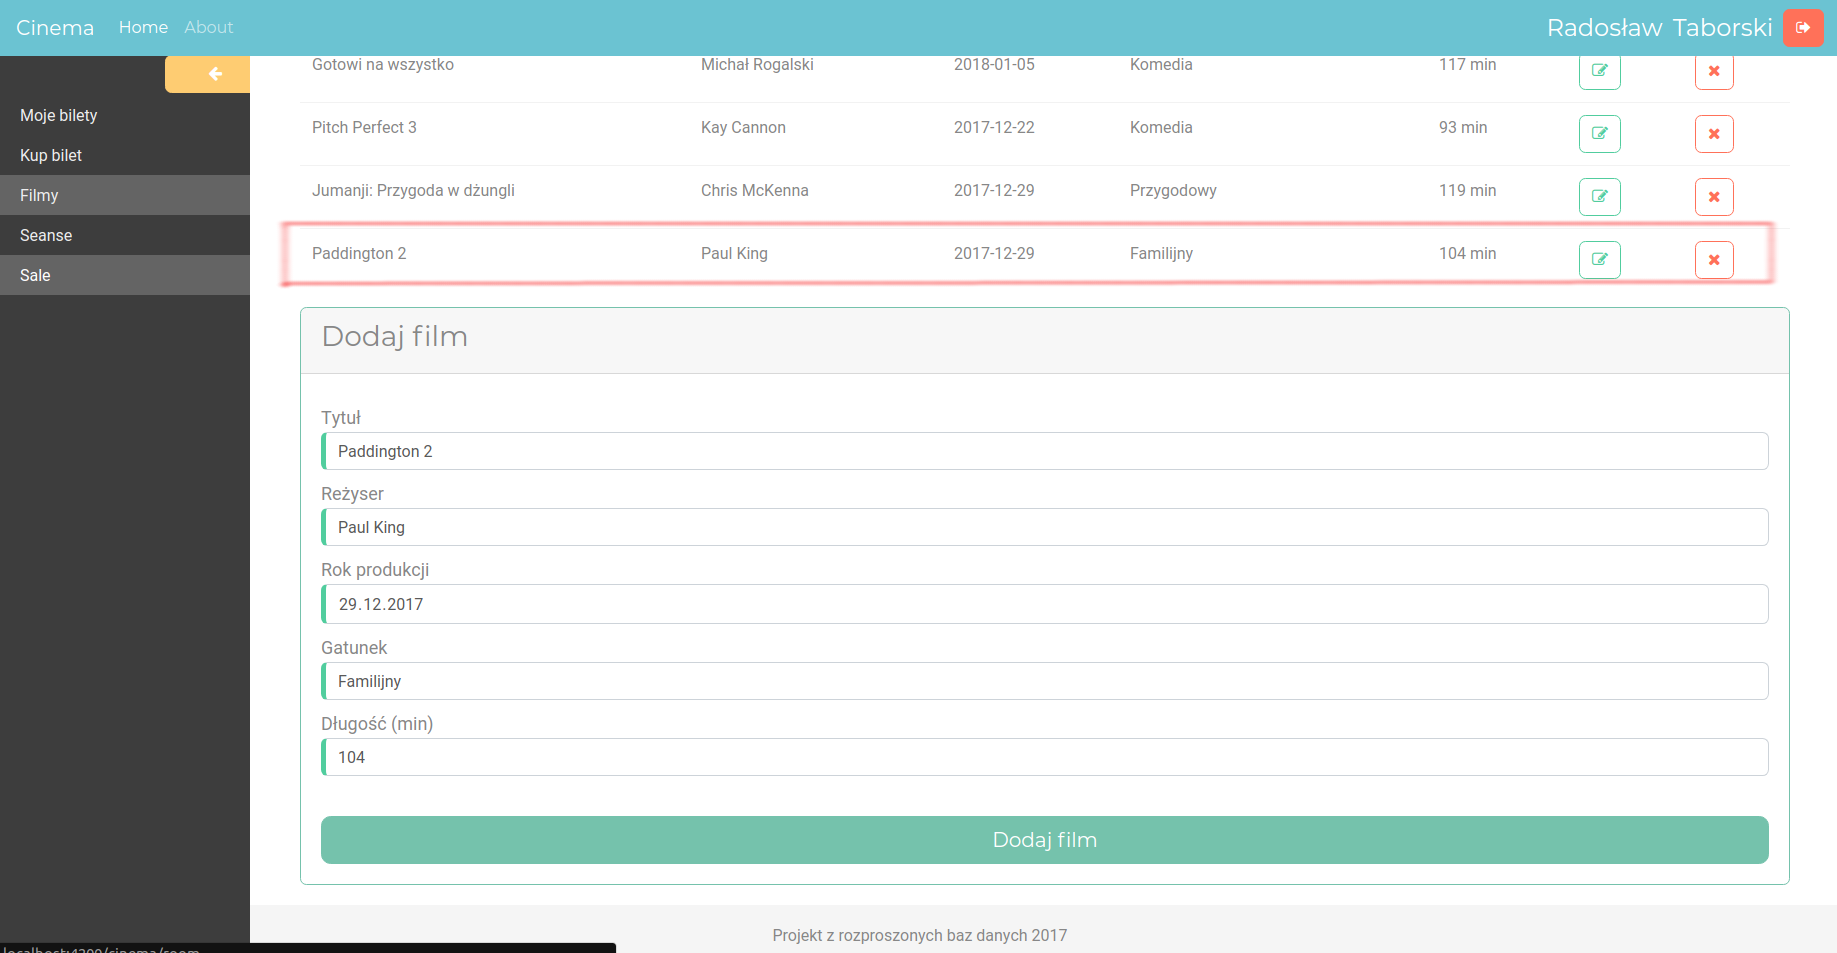
\includegraphics[width=1\linewidth]{rozdzial06/6.png}
	\caption{Nowy film wyświetlany w aplikacji}
	\label{fig:endAddFilm}
\end{figure}

\subsection{Usuwanie rekordu z rozproszonej bazy danych}

Na rysunkach od \ref{fig:removeFilm} do \ref{fig:endRemoveFilm} zademonstrowane zostało działanie replikacji na przykładzie dodawania filmu do bazy z poziomu aplikacji webowej.\\

Na rysunku \ref{fig:removeFilm} przedstawione zostały filmy znajdujące się w bazie danych wyświetlane poprzez aplikację kliencką. Będąc zalogowanym na konto administratorskie można usunąć film znajdujący się w bazie. Można tego dokonać poprzez kliknięcie czerwonego przycisku "X" obok wybranego filmu. Aplikacja wtedy łączy się poprzez API REST z węzłem master rozproszonej bazy danych, gdyż wprowadzana będzie modyfikacja, a następnie usunięty zostaje wybrany film z tabeli Filmy (rysunek \ref{fig:FilmMasterRemove}), dzięki procedurze SQL 'UsunFilm'. Wykonana procedura zostaje zreplikowana do wszystkich węzłów Slave. Tabela Filmy dla wybranego węzła Slave na porcie 8083 została pokazana na rysunku \ref{fig:FilmSlaveRemove}. Z węzła Slave również odczytywane są dane poprzez aplikację kliencką, a poprawnie odczytane dane z takiego węzła zostały przedstawione na rysunku \ref{fig:endRemoveFilm}. W przedstawionym przykładzie usunięty został film, który na rysunku~\ref{fig:FilmMaster} widoczny jest pod ID = 27. Jest to film o nazwie \textit{Jumanji: Przygoda w dżungli}.

\begin{figure} [H]
	\centering
	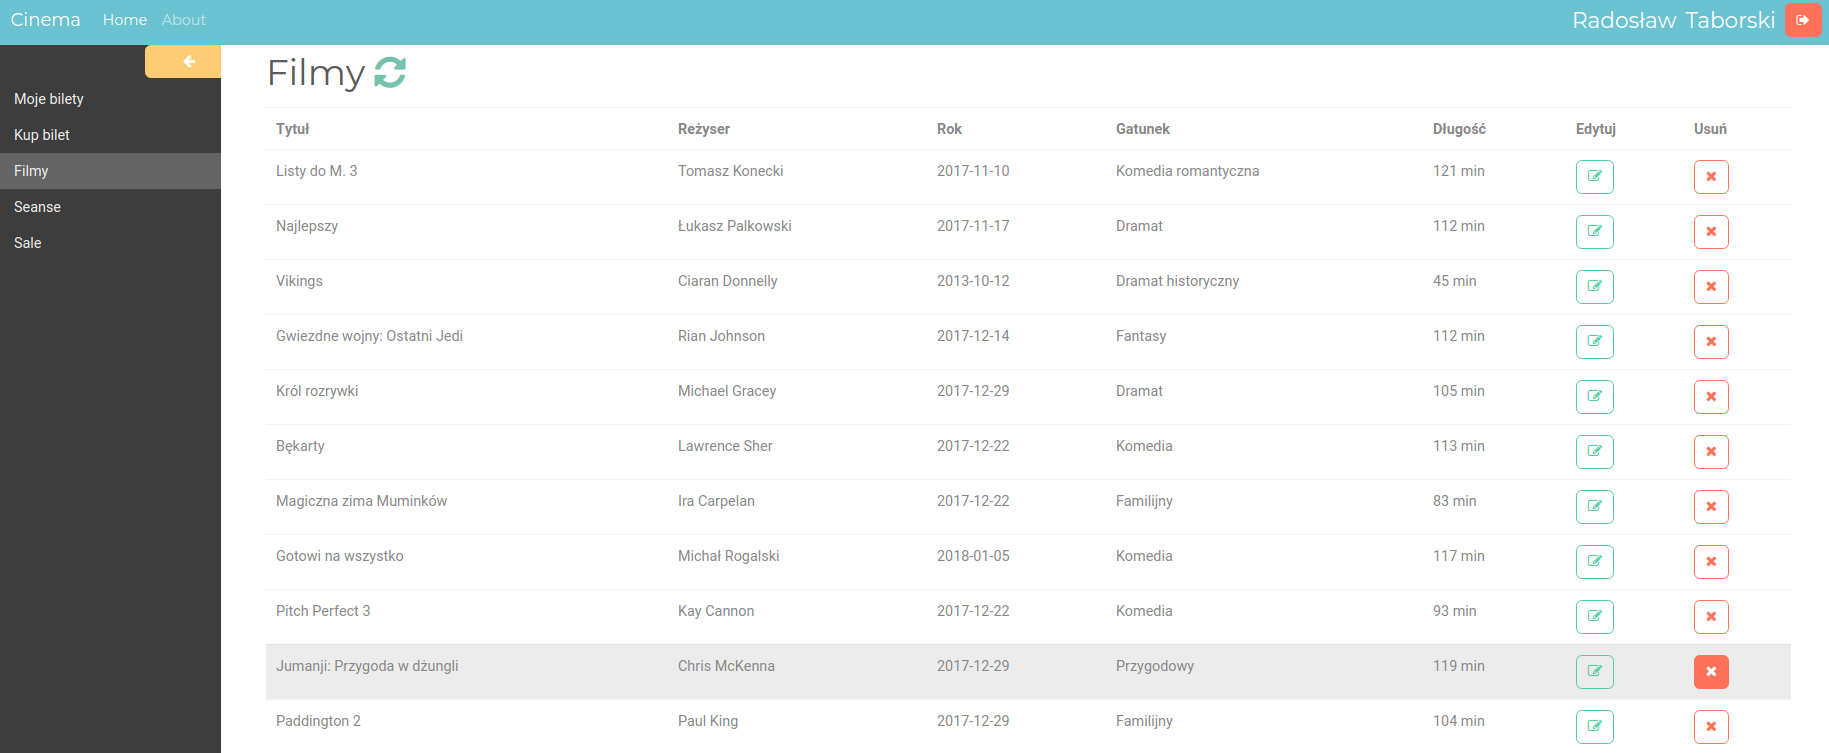
\includegraphics[width=1\linewidth]{rozdzial06/r1.png}
	\caption{Usunięcie filmu poprzez aplikację}
	\label{fig:removeFilm}
\end{figure}

\begin{figure} [H]
	\centering
	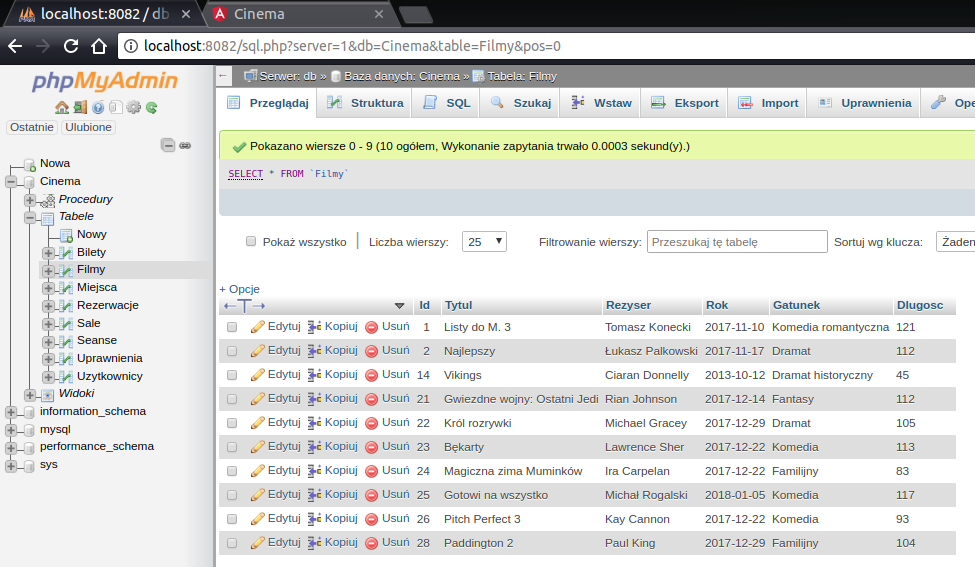
\includegraphics[width=1\linewidth]{rozdzial06/r2.png}
	\caption{Tabela Filmy na węźle \textit{master} o porcie 8082}
	\label{fig:FilmMasterRemove}
\end{figure}

\begin{figure} [H]
	\centering
	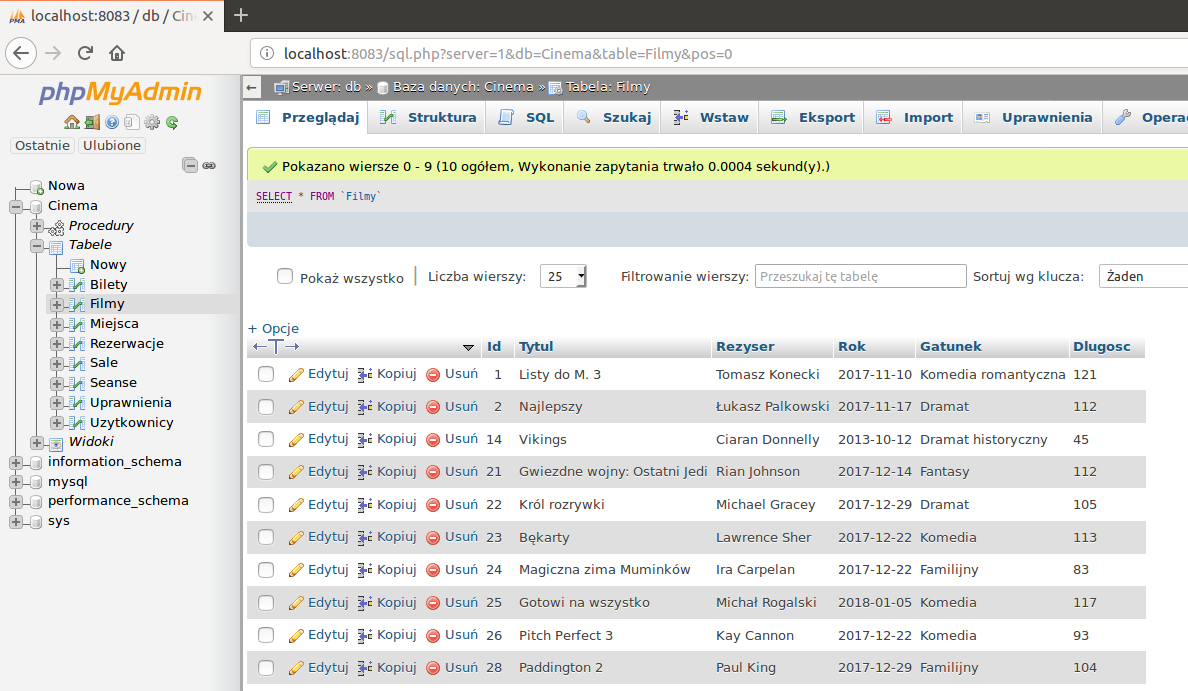
\includegraphics[width=1\linewidth]{rozdzial06/r3.png}
	\caption{Tabela Filmy na węźle \textit{slave1} o porcie 8083}
	\label{fig:FilmSlaveRemove}
\end{figure}

\begin{figure} [H]
	\centering
	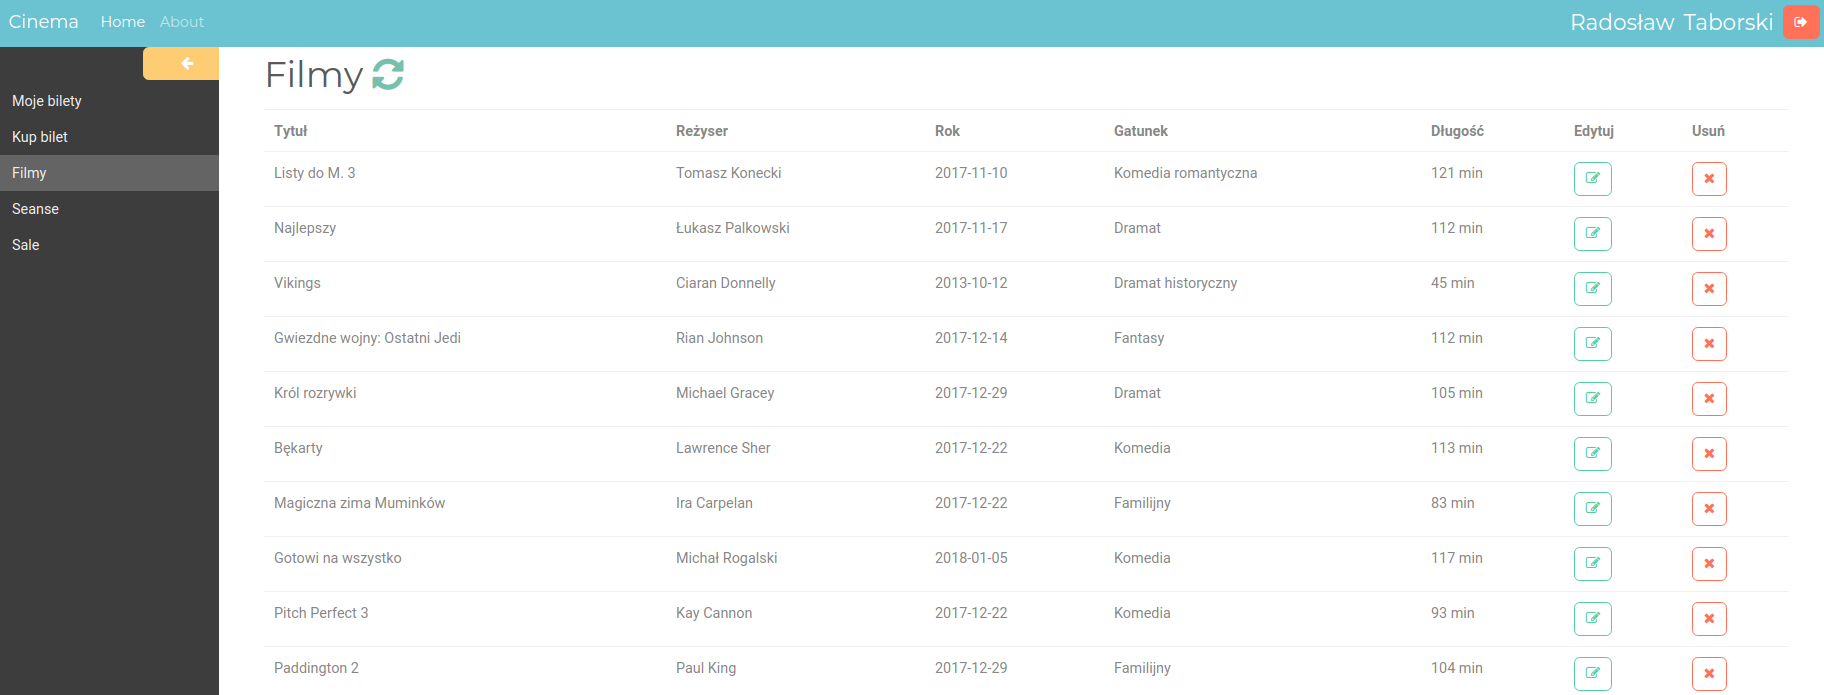
\includegraphics[width=1\linewidth]{rozdzial06/r4.png}
	\caption{Brak usuniętego filmu w aplikacji}
	\label{fig:endRemoveFilm}
\end{figure}



